

\section{Dedalus}
We take as our foundation 
%language 
an augmented version of \linebreak
$\lnot$Datalog~\cite{ullmanbook} with aggregate function
symbols akin to those of SQL (min, max, avg, stdev, count).  In general, we are interested in the classes of statically
stratifiable and locally stratifiable programs~\cite{prz}.  In addition, we admit the
use of the \emph{choice} construct~\cite{greedychoice, eventchoice} to model
nondeterministic selection of an element from a set.  
%%\jmh{save the next sentence for later.  stay pure here.}
%%In \dedalus, we will use this construct to
%%model both the nondeterminism of message delay, and the semantics of key
%%maintenance in prior deductive update models like Overlog~\cite{boon}.

%%\jmh{Can't we borrow this from somebody else rather than define it ourselves?  ``As in Ullman, et al [FOO] we represent...''}
As a matter of notation, we refer to an infinite universe of constants \emph{C}, in which
$C_{1}, C_{2}, \ldots$ are representations of individual constants, and
an infinite universe of variable symbols $A = A_1, A_2, \ldots$, and a distinguished variable $\Tau$.
% which may take on the values
% of any constants.   
We also make use of the set of positive integers $\mathbb{Z}$,
(which we will use to represent possible times), along with its natural total order
\dedalus{successor($A_i, A_j$)} and a distinguished constant symbol $\perp$ that we will use to represent ``never''.

\subsection{Syntactic Restrictions}
%%\jmh{I wonder if it wouldn't be better to do a totally syntactic definition of Dedalus as a restricted subclass of Datalog+stratification+successor, with some convenience %%notation that falls out of the restrictions.  It would ensure that we don't skip steps, and allow us to fall back on proofs about Datalog without being sloppy.  The intro %%paragraph before is only halfway formal and might be better off with a firm basis in citeable Datalog papers.}

%%A Dedalus program is a Datalog program in which every predicate is annotated with a time suffix.  \jmh{Already some slop ... you want to define it via Datalog+strat
%%+succ.  You could start by using Datalog notation but requiring the last attribute of each predicate to range over $\mathbb{Z}$, and then introduce the @-sign notation.}  
%%A Dedalus predicate has the following form:

%%$p(A_{1}, A_{2}, [...], A_{n})@S$
We will define \dedalus as a restricted sublanguage of the augmented version of $\lnot$Datalog defined above, with some notational shortcuts that fall out naturally.

Our first restriction is on the admissible schemata of our language. We  require that the final attribute of every \dedalus predicate range over the set $\mathbb{Z}$.  In a typical interpretation, \dedalus programs will use this final attribute to connote ``timestamps'', so we refer to this attribute at the \emph{time suffix} of the corresponding predicate.  

%%\wrm{we really want an inclusion constraint not just in the set of integers, but in the set of all possible times, in case time is finite}.  \jmh{I disagree, actually.  EDB facts can be sprinkled throughout time without restriction, and the rule syntax below provides the restrictions you want.  you're hinting at the reduction stuff below, but we can rewrite to that.}  

Facts are defined just as in Datalog, thus a fact
will have a constant integer value for its time suffix: e.g.


$p(C_{1},C_{2},[...],C_{n}, i) |  i \in \mathbb{Z}$

Our second and third restrictions are on rules.  
No EDB predicates may ever be referenced by rules; instead, for every EDB relation $r$ we define relations $r\_pos$ 
and $r\_neg$ with the same schema, and add a rule of the form:

$r\_pos(A_1, A_2, [...], A_n) \leftarrow r(A_1, A_2, [...], A_n);$

That is, for every EDB predicate
$r$ there is an IDB predicate $r\_pos$ that contains at least the contents of $r$.  We further restrict the
language to refer only to the EDB in distinguished rules such at that above; otherwise all rules must refer 
only to IDB predicates.
A {\em well-formed }\dedalus rule is a Datalog rule that adheres to the following constraints on body and head.  

In the rule body, every
subgoal is required to use the distinguished variable $\Tau$ as its time suffix.  
%%\jmh{I would not introduce the following constraint -- can't we have rules that fire at a particular timestep?  It may slightly complicate your reductions later, but it seems manageable.}
$\Tau$ must not be otherwise
constrained (e.g. it must not occur in the rule body except as a time suffix).
The head of a well-formed rule similarly contains a time suffix $S$, which must
be constrained in exactly one of the following three ways:

\begin{enumerate}

\item The rule is said to be \emph{deductive} if $S$ is
bound to the value $\Tau$.  That is, the body contains a subgoal of the form:
\dedalus{S = $\Tau$}.

\item The rule is said to be {\em inductive} if $S$ is the successor
of $\Tau$.  That is, the body contains a subgoal of the form:
\dedalus{successor($\Tau$, S)}.

\item The rule is said to be {\em asynchronous} if $S$ results from a non-deterministic choice function, which may be independent of $\Tau$.  We express this by adding two subgoals
to the body: \dedalus{successor(\_, $\Tau$), choose((\_), ($\Tau$))}.  The
\dedalus{choice} subgoal ensures that the $\Tau$ value projected into the head of
the rule is some arbitrary $\Tau$-value of \emph{successor}. \wrm{Why can't we
select the initial time?  What we should do instead is have some unary relation
time(T) that captures all possible times, and choose from this relation
instead.  We can assume an inclusion constraint forcing successor's arguments
to both come from this relation.}  \jmh{Good point.  OTOH I suspect we'll have to forbid messages into the past, in which case this will be fine (and succinct).}  \jmh{Actually, we should be able to express delays that are a function of attributes -- e.g. a sender-receiver pair may be input to a real-world delay distribution, as might be the time.}

\end{enumerate}

\paa{shouldn't we have an example here?}

\subsection{Extensional, Intensional and Nondeterministic Databases}

%%\jmh{Ack ... deductive rules are unsafe, and technically Datalog-neg forbids them due to the free variable in the head.  So you will need to expand your language to include an acceptable notion of per-timestep safety (as Maier suggested), at which point it's not a subset of Datalog-neg.  Would be nice to be able to say ``Dedalus is a subset of (Datalog + \{set of addons\})'' but that would require defining the acceptable saftey before defining timestamps (which are a restriction).}

\wrm{begin misplaced definitions}

Each relation in a Dedalus program is of exactly one of the three kinds:

\newdef{definition}{Definition}

%\begin{definition}
%
%A {\em Dedalus program} is a set of Dedalus rules.
%
%\end{definition}

\begin{definition}
%
An \emph{extensional} relation in a Dedalus program is a relation that does not
appear in the head of any rule in the program.
%
\end{definition}

 \begin{definition}
 %
 An \emph{intensional} relation in a Dedalus program is a relation that appears
 in the head of one or more atemporal or inductive rules in the program, but never in the head of an asynchronous rule.
 %
 \end{definition}

 \begin{definition}
 %
 A \emph{nondeterministic} relation in a Dedalus program is a relation that appears in
 the head of one or more asynchronous rules in the program.
 %
 \end{definition}

 We refer to the sets of ground atoms in extensional, intensional, and nondeterministic
 predicates respectively as the EDB, IDB, and NDB.  We will refer to facts, ground atoms
 in the EDB, and \emph{events} interchangeably, for reasons which will soon become clear.

 %\jmh{introduction of the MDB doesn't seem useful, actually.  I'd drop this, and if you need to define a ``mutable'' relation as one that participates in the head of a temporal rule, you can do so as needed.}
 The EDB, IDB, and NDB are all pairwise disjoint.  Intuitively, the distinction
 between the NDB and IDB is that the NDB is determined nondeterministically from
 the EDB, IDB and NDB, while the IDB is determined deterministically from the
 EDB, IDB and NDB.  Thus, given a Dedalus instance, all IDB
 predicates that do not transitively depend on NDB predicates can be evaluated
 deterministically.  
 %%\jmh{The only reason to worry about the MDB being non-deterministic is @sync, which you didn't in fact need to introduce yet.  Again, I don't see this discussion being useful.}


\begin{figure}[t]
  \centering
  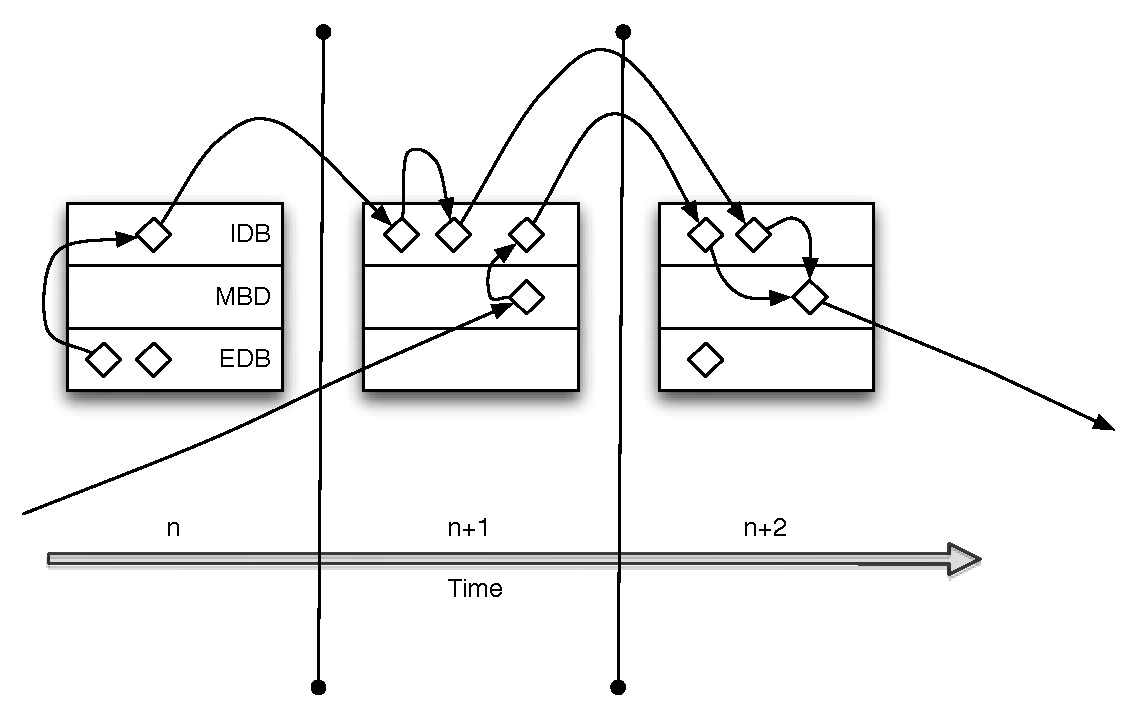
\includegraphics[width=1\linewidth]{edbidbmdb.pdf}
  \label{fig:edbidbmdb}
  \caption{Derivations across time in IDB and MDB relations.}
\vspace{-8pt}
\end{figure}




\subsection{Abbreviated Syntax and Temporal Interpretation}
We have been careful to define Dedalus as a syntactic subset of a natural variant of Datalog; this allows us to take advantage of Datalog's well-known semantics and the rich literature on the language.  

However Dedalus programs are intended to capture naturally temporal semantics.  For example, a fact with some constant $C_i$ in its time suffix can be thought of as a fact that is true ``at time $C_i$''.  Deductive rules can be seen as {\em atemporal} statements: they range over all values of the time suffix, and express deductions that are ``always'' valid.
Inductive and asynchronous rules are {\em temporal}:
their consequents are defined to be true ``at a different time'' than their antecedents. 

To simplify Dedalus notation for this typical interpretation,  we introduce some natural syntactic ``sugar'' as follows:  

\begin{itemize}
	\item {\em Time-suffix notation:}  The final, time-suffix attribute of each predicate is placed after the predicate's right parenthesis, separated by the symbol `@'.   For example, the predicate \\
	$r(A_{1}, \ldots, A_{n}, S)$ is rewritten as $r(A_{1}, \ldots, A_{n})@S$.
	\item {\em Implicit time-suffixes in body predicates:} Since all body predicates of a well-formed rule have a free variable $\Tau$ in the time suffix, we omit the time suffix from body predicates and treat it as implicit. 
	\item {\em Temporal head annotation:} The inclusion of the \emph{successor}
and \emph{choice} predicates in the body is promoted to a keyword in the time suffix of the head predicate, in the form:

$r(A_{1},A_{2},[...],A_{n})@S$

where $S$ is one of the following:
\begin{enumerate}
\item \emph{now}: a deductive rule, in which all predicates implicitly share the same time suffix $\Tau$.
\item \emph{next}: an inductive rule, in which the \emph{successor($\Tau$, S)} predicate is implicitly included in the body as described above, and $S$ is implicitly the time suffix of the head
\item \emph{async(N)}: an asynchronous rule, in which the time suffix of the head predicate will occur some time after the time suffix of the body predicate, or never.
N is a variable, corresponding to the time suffix $\Tau$ of all predicates in the rule body and optionally referenced in the head.
%in which the time suffix of the head predicate is implicitly chosen nondeterministically via choice as described above.
%wrm: chosen via choice is too operational.
\end{enumerate}
\end{itemize}

% \jmh{the following is redundant and can be omitted}
% Dedalus facts are just datalog facts that conform to the schema constraint:  rule heads with empty bodies, and ground terms for all attributes including the time suffix.  To accommodate this in our notation,
% we allow a fourth suffix for the special case of empty bodies: a constant integer.  A Dedalus fact thus has the form:
% 
% $r(C_1, C_2, [...], C_n)@CI$
% 
% where $CI$ is an integer constant.


%Finally, we define the following shorthand for referring to the special IDB relations defined above.  Recall that for every EDB predicate $r$
%we have a uniquely defined pair of IDB predicates $r\_pos$ and $r\_neg$.  In a Dedalus program, we use $r$ as shorthand for $r\_pos$ 
%(recall that the true EDB predicate $r$ cannot be referenced by any rules) and $delete$ $r$ as shorthand for $r\_neg$.
%%A deductive rule as defined above will hold for any assignment of a constant integer to the $N$-value in the suffix of each predicate.

%%\subsection{Events}

%%\newdef{definition}{Definition} 
%%\begin{definition}
%
%%An \emph{event} in Dedalus is an EDB fact.
%
%%\end{definition}

%%\jmh{Isn't the following simply a restatement of Datalog's use of EDB?}
%%Since an extensional relation may not appear in a rule's head, events come from
%%sources external to the evaluation of the Dedalus instance.

